\documentclass[11pt, oneside]{article}   	% use "amsart" instead of "article" for AMSLaTeX format
\usepackage{geometry}                		% See geometry.pdf to learn the layout options. There are lots.
\geometry{letterpaper}                   		% ... or a4paper or a5paper or ... 
%\geometry{landscape}                		% Activate for rotated page geometry
%\usepackage[parfill]{parskip}    		% Activate to begin paragraphs with an empty line rather than an indent
\usepackage{graphicx}				% Use pdf, png, jpg, or eps§ with pdflatex; use eps in DVI mode
								% TeX will automatically convert eps --> pdf in pdflatex		
\usepackage{amssymb}
\usepackage{tikz}
\usetikzlibrary{arrows,positioning,calc,shapes.geometric}
%SetFonts

%SetFonts


\title{Brief Article}
\author{The Author}
%\date{}							% Activate to display a given date or no date

\begin{document}
%\maketitle
%\section{}
%\subsection{}

{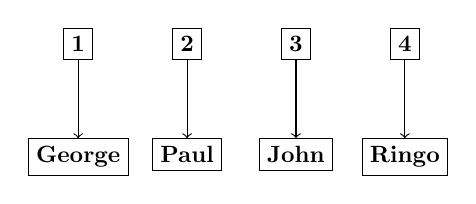
\begin{tikzpicture}[auto, scale=1, every node/.style={scale=.85}, node distance=1]
    \node (n1) at (0,0) [rectangle, draw] {{\centering \bf{1}} };%\bf Blackboard};
  \node (n2) [right=of n1, rectangle, draw] {{\centering \bf{2} }};
  \node (n3) [right=of n2, rectangle, draw] {{\centering \bf{3} }};
  \node (n4) [right=of n3, rectangle, draw] {{\centering \bf{4} }};
  \node (bg) [below=of n1, rectangle, draw] {{\centering \bf{George} }};
  \node (bp) [right=of bg, below=of n2, rectangle, draw] {{\centering \bf{Paul} }};
  \node (bj) [right=of bp, below=of n3, rectangle, draw] {{\centering \bf{John} }};
  \node (br) [right=of bj, below=of n4, rectangle, draw] {{\centering \bf{Ringo} }};
  \draw[->] (n1) to node {} (bg);
  \draw[->] (n2) to node {} (bp);
  \draw[->] (n3) to node {} (bj);
  \draw[->] (n4) to node {} (br);
\end{tikzpicture}}

\vspace{2cm}

{\begin{tikzpicture}[auto, scale=1, every node/.style={scale=.85}, node distance=1]
    \node (n1) at (0,0) [rectangle, draw] {{\centering \bf{1}} };%\bf Blackboard};
  \node (n2) [right=of n1, rectangle, draw] {{\centering \bf{2} }};
  \node (n3) [right=of n2] {{\centering $\ldots$ }};
  \node (n4) [right=of n3, rectangle, draw] {{\centering $n$ }};
  \node (n5) [right=of n4] {{\centering $\ldots$ }};
  \node (bg) [below=of n1, rectangle, draw] {{\centering $a$ }};
  \node (bp) [right=of bg, below=of n2, rectangle, draw] {{\centering $b$ }};
  \node (bd1) [right=of bp, below=of n3] {{\centering $\ldots$}};
  \node (bj) [right=of bp, below=of n4, rectangle, draw] {{\centering $q$ }};
  \node (bd2) [right=of bp, below=of n5] {{\centering $\ldots$}};
%  \node (br) [right=of bj, below=of n4, rectangle, draw] {{\centering \bf{Ringo} }};
  \draw[->] (n1) to node {} (bg);
  \draw[->] (n2) to node {} (bp);
%  \draw[->] (n3) to node {} (bj);
  \draw[->] (n4) to node {} (bj);
\end{tikzpicture}}


\vspace{2cm}

{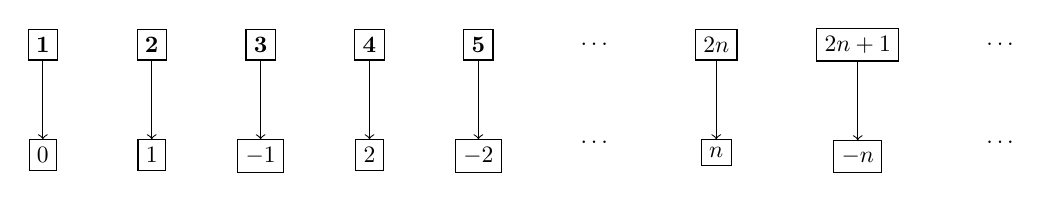
\begin{tikzpicture}[auto, scale=1, every node/.style={scale=.85}, node distance=1]
    \node (n1) at (0,0) [rectangle, draw] {{\centering \bf{1}} };%\bf Blackboard};
  \node (n2) [right=of n1, rectangle, draw] {{\centering \bf{2} }};
  \node (n3) [right=of n2, rectangle, draw] {{\centering \bf{3} }};
  \node (n4) [right=of n3, rectangle, draw] {{\centering \bf{4} }};
  \node (n5) [right=of n4, rectangle, draw] {{\centering \bf{5} }};
  \node (nd) [right=of n5] {{\centering $\ldots$ }};
  \node (nn) [right=of nd, rectangle, draw] {{\centering $2n$ }};
  \node (nn1) [right=of nn, rectangle, draw] {{\centering $2n+1$ }};
  \node (nd1) [right=of nn1] {{\centering $\ldots$ }};
  \node (b0) [below=of n1, rectangle, draw] {{\centering \bf{$0$} }};
  \node (b1) [right=of b0, below=of n2, rectangle, draw] {{\centering \bf{$1$} }};
  \node (b2) [right=of b1, below=of n3, rectangle, draw] {{\centering \bf{$-1$} }};
  \node (b3) [right=of b2, below=of n4, rectangle, draw] {{\centering \bf{$2$} }};
  \node (b4) [right=of b3, below=of n5, rectangle, draw] {{\centering \bf{$-2$} }};
  \node (bd) [right=of b4, below=of nd] {{\centering $\ldots$}};
  \node (bn) [right=of bd, below=of nn, rectangle, draw] {{\centering $n$ }};
  \node (bn1) [right=of bn, below=of nn1, rectangle, draw] {{\centering $-n$ }};
  \node (bd1) [right=of bn1, below=of nd1] {{\centering $\ldots$}};
%  \node (br) [right=of bj, below=of n4, rectangle, draw] {{\centering \bf{Ringo} }};
  \draw[->] (n1) to node {} (b0);
  \draw[->] (n2) to node {} (b1);
  \draw[->] (n3) to node {} (b2);
  \draw[->] (n4) to node {} (b3);
  \draw[->] (n5) to node {} (b4);
  \draw[->] (nn) to node {} (bn);
  \draw[->] (nn1) to node {} (bn1);
\end{tikzpicture}}

\vspace{2cm}

{\begin{tikzpicture}[auto, scale=1, every node/.style={scale=.85}, node distance=1]
    \node (n11) at (0,0) {\centering  $\frac{1}{1}$};
    \node (n12) [right=of n11] {\centering  $\frac{1}{2}$};
    \node (n13) [right=of n12] {\centering  $\frac{1}{3}$};
    \node (n14) [right=of n13] {\centering  $\frac{1}{4}$};
    \node (n15) [right=of n14] {\centering  $\frac{1}{5}$};
    \node (d1) [right=of n15] {\centering $\ldots$};
    
    \node (n21) [below=of n11] {\centering  $\frac{2}{1}$};
    \node (n22) [right=of n21] {\centering  $\frac{2}{2}$};
    \node (n23) [right=of n22] {\centering  $\frac{2}{3}$};
    \node (n24) [right=of n23] {\centering  $\frac{2}{4}$};
    \node (n25) [right=of n24] {\centering  $\frac{2}{5}$};
    \node (d2) [right=of n25] {\centering $\ldots$};
    
    \node (n31) [below=of n21] {\centering  $\frac{3}{1}$};
    \node (n32) [right=of n31] {\centering  $\frac{3}{2}$};
    \node (n33) [right=of n32] {\centering  $\frac{3}{3}$};
    \node (n34) [right=of n33] {\centering  $\frac{3}{4}$};
    \node (n35) [right=of n34] {\centering  $\frac{3}{5}$};
    \node (d3) [right=of n35] {\centering $\ldots$};
    
    \node (n41) [below=of n31] {\centering  $\frac{4}{1}$};
    \node (n42) [right=of n41] {\centering  $\frac{4}{2}$};
    \node (n43) [right=of n42] {\centering  $\frac{4}{3}$};
    \node (n44) [right=of n43] {\centering  $\frac{4}{4}$};
    \node (n45) [right=of n44] {\centering  $\frac{4}{5}$};
    \node (d4) [right=of n45] {\centering $\ldots$};
    
    \node (n51) [below=of n41] {\centering  $\frac{5}{1}$};
    \node (n52) [right=of n51] {\centering  $\frac{5}{2}$};
    \node (n53) [right=of n52] {\centering  $\frac{5}{3}$};
    \node (n54) [right=of n53] {\centering  $\frac{5}{4}$};
    \node (n55) [right=of n54] {\centering  $\frac{5}{5}$};
    \node (d5) [right=of n55] {\centering $\ldots$};   
    
    \node (n61) [below=of n51] {\centering  $\vdots$};
    \node (n62) [right=of n61] {\centering  $\vdots$};
    \node (n63) [right=of n62] {\centering  $\vdots$};
    \node (n64) [right=of n63] {\centering  $\vdots$};
    \node (n65) [right=of n64] {\centering  $\vdots$};
 %   \node (d5) [right=of n55] {\centering $\ldots$};
 
\end{tikzpicture}}

\vspace{2cm}

{\begin{tikzpicture}[auto, scale=1, every node/.style={scale=.85}, node distance=1]
    \node (n11) at (0,0) {\centering  $\frac{1}{1}$};
    \node (n12) [right=of n11] {\centering  $\frac{1}{2}$};
    \node (n13) [right=of n12] {\centering  $\frac{1}{3}$};
    \node (n14) [right=of n13] {\centering  $\frac{1}{4}$};
    \node (n15) [right=of n14] {\centering  $\frac{1}{5}$};
    \node (d1) [right=of n15] {\centering $\ldots$};
    
    \node (n21) [below=of n11] {\centering  $\frac{2}{1}$};
    \node (n22) [right=of n21] {\centering  $\frac{2}{2}$};
    \node (n23) [right=of n22] {\centering  $\frac{2}{3}$};
    \node (n24) [right=of n23] {\centering  $\frac{2}{4}$};
    \node (n25) [right=of n24] {\centering  $\frac{2}{5}$};
    \node (d2) [right=of n25] {\centering $\ldots$};
    
    \node (n31) [below=of n21] {\centering  $\frac{3}{1}$};
    \node (n32) [right=of n31] {\centering  $\frac{3}{2}$};
    \node (n33) [right=of n32] {\centering  $\frac{3}{3}$};
    \node (n34) [right=of n33] {\centering  $\frac{3}{4}$};
    \node (n35) [right=of n34] {\centering  $\frac{3}{5}$};
    \node (d3) [right=of n35] {\centering $\ldots$};
    
    \node (n41) [below=of n31] {\centering  $\frac{4}{1}$};
    \node (n42) [right=of n41] {\centering  $\frac{4}{2}$};
    \node (n43) [right=of n42] {\centering  $\frac{4}{3}$};
    \node (n44) [right=of n43] {\centering  $\frac{4}{4}$};
    \node (n45) [right=of n44] {\centering  $\frac{4}{5}$};
    \node (d4) [right=of n45] {\centering $\ldots$};
    
    \node (n51) [below=of n41] {\centering  $\frac{5}{1}$};
    \node (n52) [right=of n51] {\centering  $\frac{5}{2}$};
    \node (n53) [right=of n52] {\centering  $\frac{5}{3}$};
    \node (n54) [right=of n53] {\centering  $\frac{5}{4}$};
    \node (n55) [right=of n54] {\centering  $\frac{5}{5}$};
    \node (d5) [right=of n55] {\centering $\ldots$};   
    
    \node (n61) [below=of n51] {\centering  $\vdots$};
    \node (n62) [right=of n61] {\centering  $\vdots$};
    \node (n63) [right=of n62] {\centering  $\vdots$};
    \node (n64) [right=of n63] {\centering  $\vdots$};
    \node (n65) [right=of n64] {\centering  $\vdots$};
 %   \node (d5) [right=of n55] {\centering $\ldots$};
 
   \draw[->] (n11) to node {} (n12);
  \draw[->] (n12) to node {} (n22);
  \draw[->] (n22) to node {} (n21);
  \draw[->] (n21) to node {} (n31);
  \draw[->] (n31) to node {} (n32);
  \draw[->] (n32) to node {} (n33);
  \draw[->] (n33) to node {} (n23); 
   \draw[->] (n23) to node {} (n13);
  \draw[->] (n13) to node {} (n14);
  \draw[->] (n14) to node {} (n24);
  \draw[->] (n24) to node {} (n34);
  \draw[->] (n34) to node {} (n44);
  \draw[->] (n44) to node {} (n43);
  \draw[->] (n43) to node {} (n42);
  \draw[->] (n42) to node {} (n41);
    \draw[->] (n41) to node {} (n51);
  \draw[->] (n51) to node {} (n52);
  \draw[->] (n52) to node {} (n53);
  \draw[->] (n53) to node {} (n54);
  \draw[->] (n54) to node {} (n55);
  \draw[->] (n55) to node {} (n45);
  \draw[->] (n45) to node {} (n35);
  \draw[->] (n35) to node {} (n25);
  \draw[->] (n25) to node {} (n15);
  \draw[->] (n15) to node {} (d1);
\end{tikzpicture}}

\end{document}  